\makeatletter
\renewcommand{\fnum@figure}{Figure \thefigure}
\makeatother

\chapter{Experiments} \label{chap:experiments}

To identify whether the Dirichlet Multinomial Regression method proposed can provide richer and more valuable information than single-output or deterministic methods can alone, we ran experiments on the data obtained from the ACFR's Sirius AUV and Schmidt's Falkor. The main machine learning algorithms' performance which we tested were Gaussian Process Classification, and Dirichlet Multinomial Regression. In this section, the experiments were designed to display the benefits of a Gaussian Process Classifier's probabilistic output, as well as the label distributions of a Dirichlet Multinomial Regressor.

\section{Mathematical Background}
\todo{(this needs/should be in its own chapter)}

\subsection{Gaussian Processes}

\todo {GP equations, description}

\todo {GP approximation methods}

\subsection{Dirichlet Multinomial Regression}

Dirichlet multinomial regression, as the name suggestions, combines dirichlet and multinomial distributions to achieve the combined model. In particular, we are interested in modeling a distribution over category counts, as there exists relationship in our data such that every bathmetry point corresponds to a certain count of each possible label in the relevant area of benthos. \todo{explain why we should first revisit dirichlet, multinomial distributions separately before looking at dirichlet multinomial regression}

\subsubsection{Multinomial Distribution}
\todo {equations, description}

\subsubsection{Dirichlet Distribution}
\todo{descriptions}

$$\theta \sim Dir(\alpha) \text{ , dirichlet distributed random variable}$$ 
$$p(\theta)= \frac{1}{\beta(\alpha)} \Pi_{i=1}^n \theta_i^{\alpha_i - 1} I(\theta \in S) \text{ density function, I is indicator function}$$ 
$$ \theta = (\theta_1, ..., \theta_n), \alpha = (\alpha_1,...,\alpha_n), \alpha_i > 0 \text{ theta - n-dimensional vectors, alpha - parameters for distribution}$$
$$ S = \{x \in R^n : x_i \geq 0, \sum x_i = 1\} \text{ S is probability simplex, the set of pmfs on numbers 1 through n}$$ 
$$\frac{1}{\beta(\alpha)} = \frac{\Gamma(\alpha_0)}{\Gamma(\alpha_i) ... \Gamma(\alpha_n)}, \alpha_0 = \sum_{i=1}^n \alpha_i \text{ generalised beta function}$$

\subsubsection{Dirichlet Multinomial Regression}

\todo{descriptions}

$$DM(C|\alpha) = \frac{M!}{\Pi_k C_k!} \frac{\Gamma(\sum_k \alpha_k)}{\Gamma(\sum_k c_k + \alpha_k)} \Pi_{k=1}^k \frac{\Gamma(C_k + \alpha_k)}{\Gamma(\alpha_k)}$$
$$ M = \sum_k c_k $$

For the regressor, the two activation functions that were considered were exponential and softmax, where the former often provided better mapping predictions, but the latter is preferable in the general case due to its better numerical stability \todo {include graphs of exponential and softmax here}.
$$\alpha_k = \exp\{x^T w_k\}$$
$$\alpha_k = \text{softmax}\{x^T w_k\}$$

The weights $w$ here are in fact a matrix of weights with dimensions $(K \times D)$, where $K$ is the number of possible labels across the dataset, and $D$ is the dimensionality of the dataset. Muliplying the dirichlet multinomial prior by the likelihood then then gives the equation over which to optimise to predict the normalised label counts at any given point.

This gives the joint-log-likelihood over both the dirichlet and multinomial distributions:
\begin{multline}
    \sum^N_{n=1} [\log(M_k) - \sum_k \log(c_k!) + \log \Gamma(\sum_k \alpha_k(x_n)) - \log \Gamma(\sum_k c_{nk} + \alpha_k(x_n))] \\
    + \sum^N_{n=1} \sum^K_{k=1} [\log \Gamma(c_k + \alpha(x)) - \log \Gamma(\alpha_k(x_n))] \\
    + \sum^K_{k=1} [-\frac{\phi}{2} \log(2\pi \phi) - \frac{1}{2}w_k^T \phi \mathbb{I} w_k]
\end{multline}

To optimise this equation, the partial derivative of the above over the weights $w$ are considered:
\begin{multline}
    \partial \frac{\log p(c, x)}{\partial w_k} = \sum_{n=1}^N x_n \alpha_k (x_n) [\psi(\sum_l \alpha_l(x_n)) - \psi(\sum_k c_{nk} + \alpha_k(x_n))] \\
    + \sum^N_{n=1} x_n \alpha_k (x_n) [\psi (c_{nk} + \alpha_k(x_n)) - \psi(\alpha_k(x_n))] - \frac{1}{\phi} w_k
\end{multline}

\todo {explain all the symbols here}

\section{Preprocessing}

\subsection{Downsampling the Data}
As the purpose of using Dirichlet Multinomial Regression was to be able to model the distribution of habitat label occurrences over an area, we downsampled the combined 2011+2015 dataset which was at a siginficantly higher resolution than the 2009 dataset. Two methods of downsampling in particular were tested. The first coarser approach involved simply taking the space in which the data was collected and placing grids of fixed size over them as in \cref{fig:gridsplit}, binning all points falling within each grid into a single datapoint. Each of these data points contained multiple points from the original dataset with their own counts for each of the possible labels, so the downsampled points simply took the sum of all the label counts in each fixed grid. 

The second summed label counts in the same way, but clusters were instead formed by first calculating the full dendrogram on the 16502 entries in the training data, and forming groups such that none had more than 5 of the original points within them, and the sub-clusters (at each level of the dendrogram) were no more than a 21 metres away from one another. As can be seen in \cref{fig:dendrogram}, the gradual merging into the single supercluster was quite consistent, indicating the original datapoints were mostly evenly distributed.

For a fair comparison between Gaussian process classification and dirichlet multinomial regression, the downsampled data was used to train the GPs as well - although this seems like an unnecessary handicap to the GP, it is more appropriate considering that one of the aims here is to demonstrate what sort of information can be gained from a DM vs. a GP, given the same \textit{raw} data.

\begin{figure}[H]
    \includegraphics[scale=0.7]{training_map_fixedgrid.pdf}
    \caption{\todo{create} Fixed-sized grids placed over training data}
    \label{fig:gridsplit}
\end{figure} 
\begin{figure}[H]
    \centering
    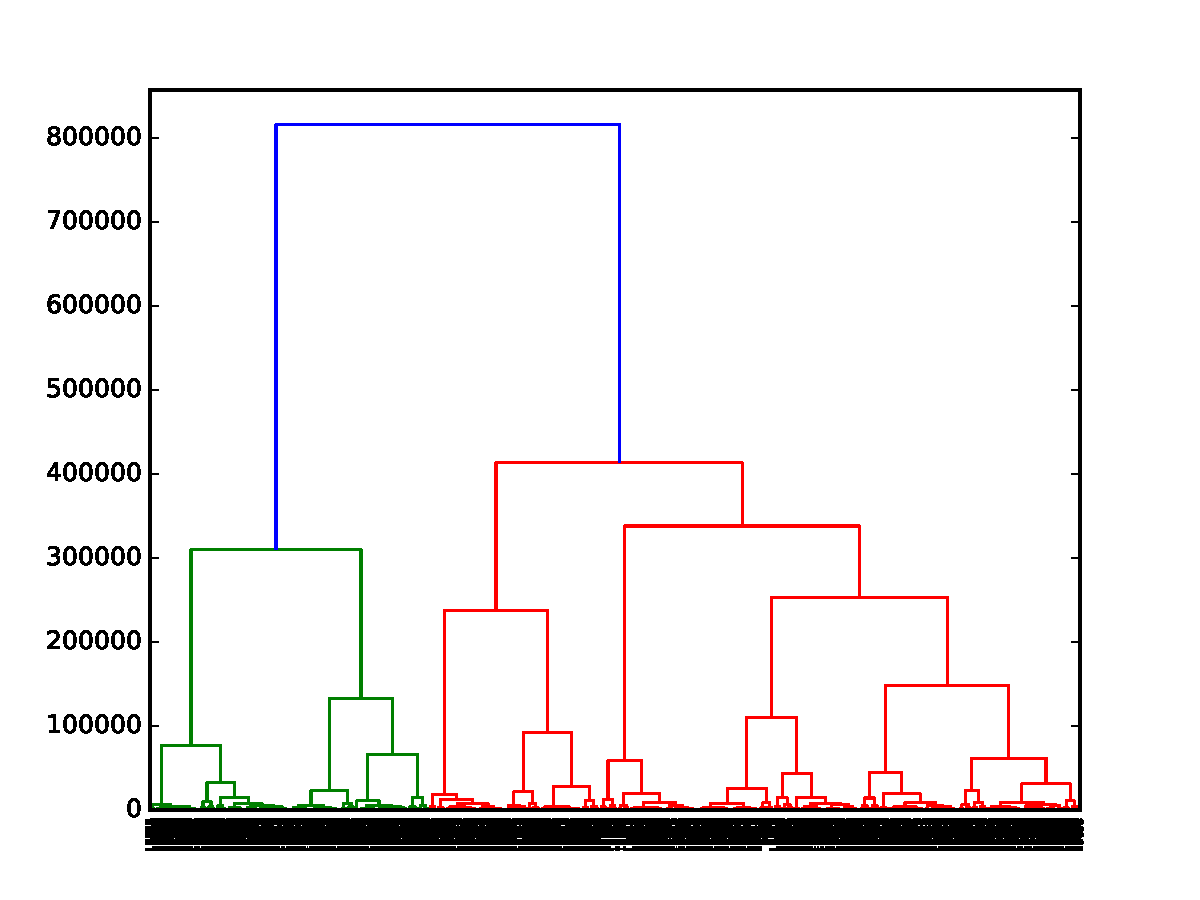
\includegraphics[scale=0.6]{dendrogram.pdf}
    \caption{Dendrogram of training data}
    \label{fig:dendrogram}
\end{figure}

\subsection{Simplifying labels}
Another step that was considered during experiments was the aggregation of habitat labels. The original training data contained 24 separate labels determined through an automated clustering procedure using Dirichlet Processes. Because of the uneven distribution of these labels(\todo{generate these images} \ref{fig:singlelabeldistr} and \ref{fig:multilabeldistr}), with the occurrence of some too insignificant for any machine learning algorithms to pick up, they were simplified in collaboration with ecological experts, who manually identified which of the 24 labels were in fact of the same class - for example, 5 separate classes of coral may have been indistinguishable to the average person, and were hence grouped into a single label. This allowed the near-non-occurring labels to be grouped together with more commonly occurring ones, whilst also allowing a different level of granularity in training models/forming predictions that could be used if only a rough approximation of an area's benthic map were required.

\todo{label mappings - give the labels for the simplified classes, e.g. coral, etc.}

\begin{tabular}{|c| c|}
    \hline
    simplified & original \\\hline
    0 & 1, 2, 18, 20, 21, 23, 24 \\
    1 & 3, 5, 10, 16, 17, 19, 22\\
    2 & 13, 14, 15 \\
    3 & 4, 6, 7, 8, 9, 11, 12 \\
    \hline
\end{tabular}

\todo{put some images here from both original and simplified classes. don't use squidle's downloader, visit server directory and d/l from there directly, 100x+ faster}

\begin{figure}[H]
    \begin{minipage}{.49\linewidth}
        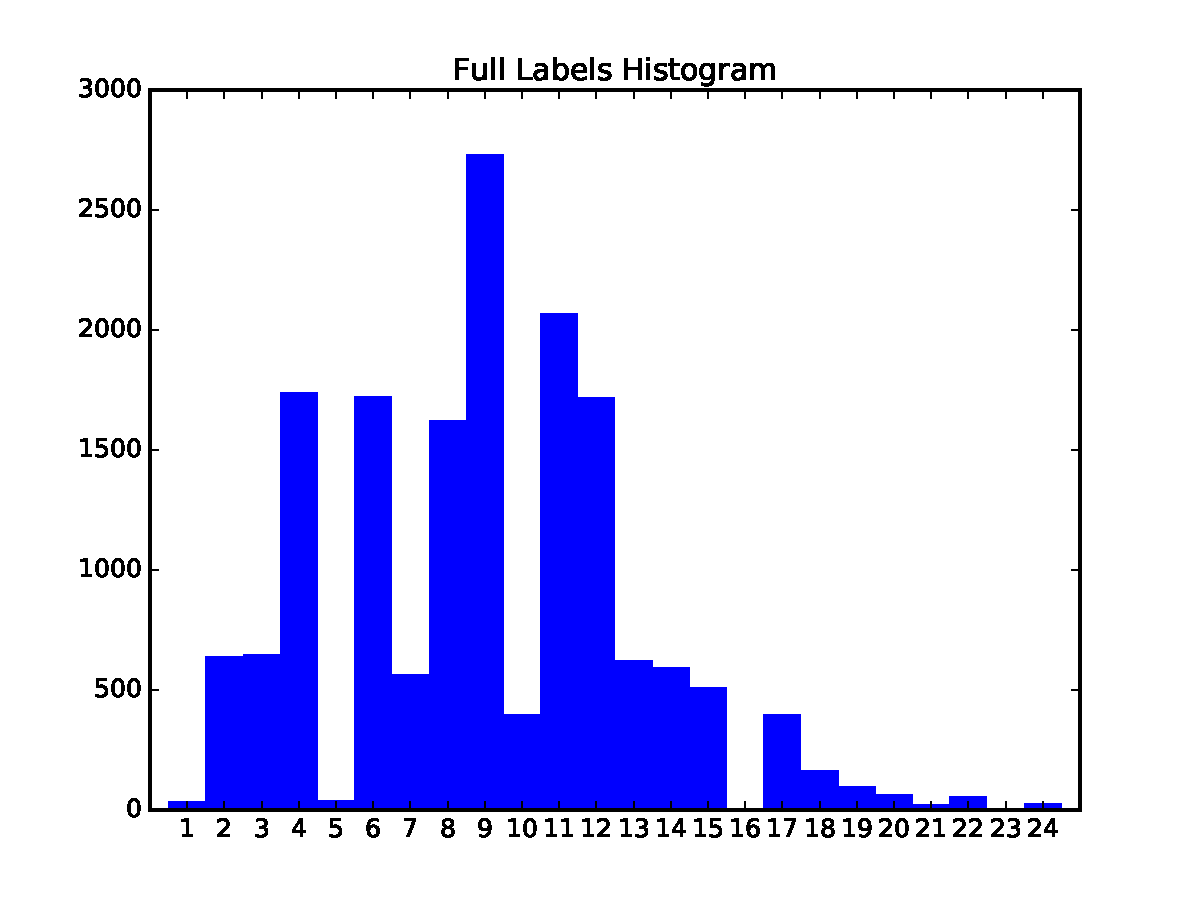
\includegraphics[width=\linewidth]{hist_full_labels.pdf}
        \caption{Distribution of labels in original dataset}
        \label{fig:singlelabeldistr}
    \end{minipage}
    \hfill
    \begin{minipage}{.49\linewidth}
        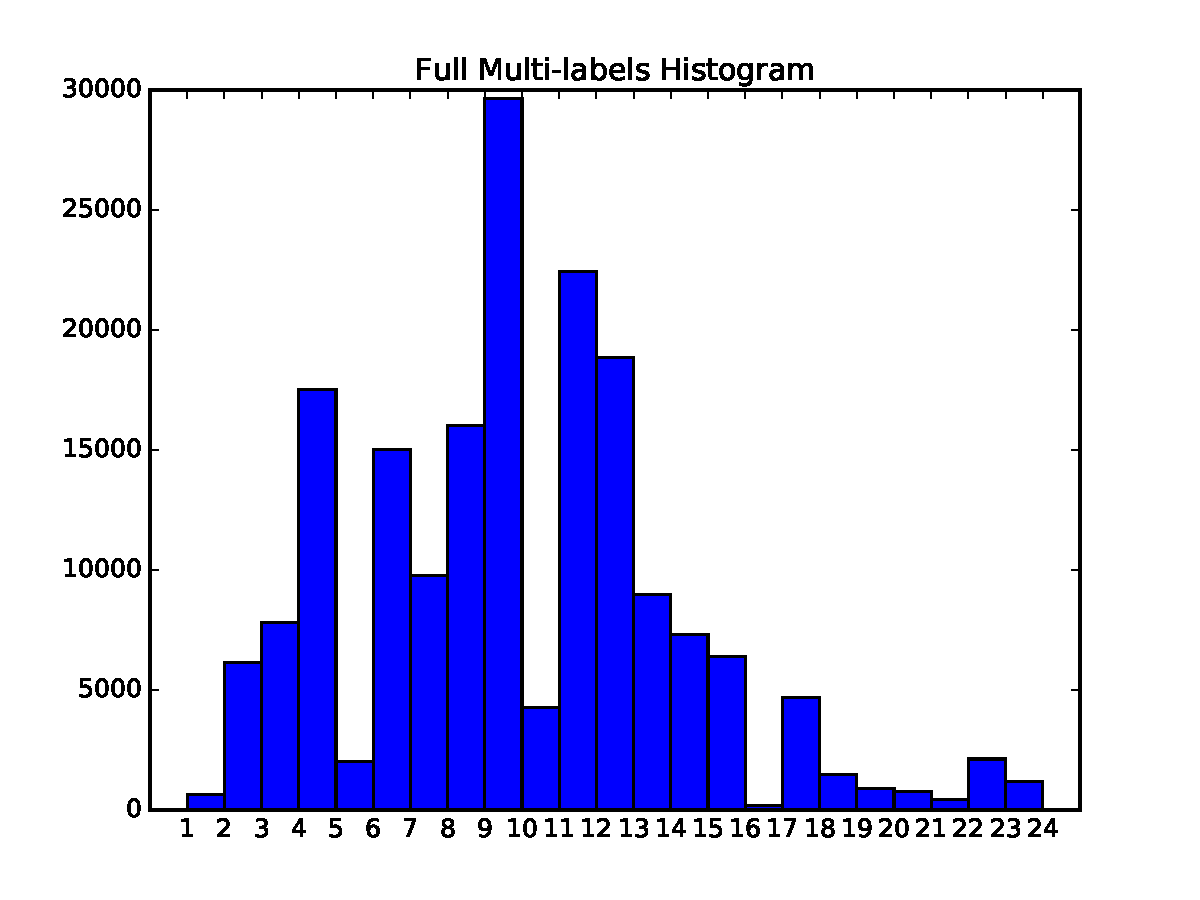
\includegraphics[width=\linewidth]{hist_full_multi_labels.pdf}
        \caption{Distribution of labels in multi-label outputs}
        \label{fig:multilabeldistr}
    \end{minipage}
\end{figure}

\begin{figure}[H]
    \begin{minipage}{.49\linewidth}
        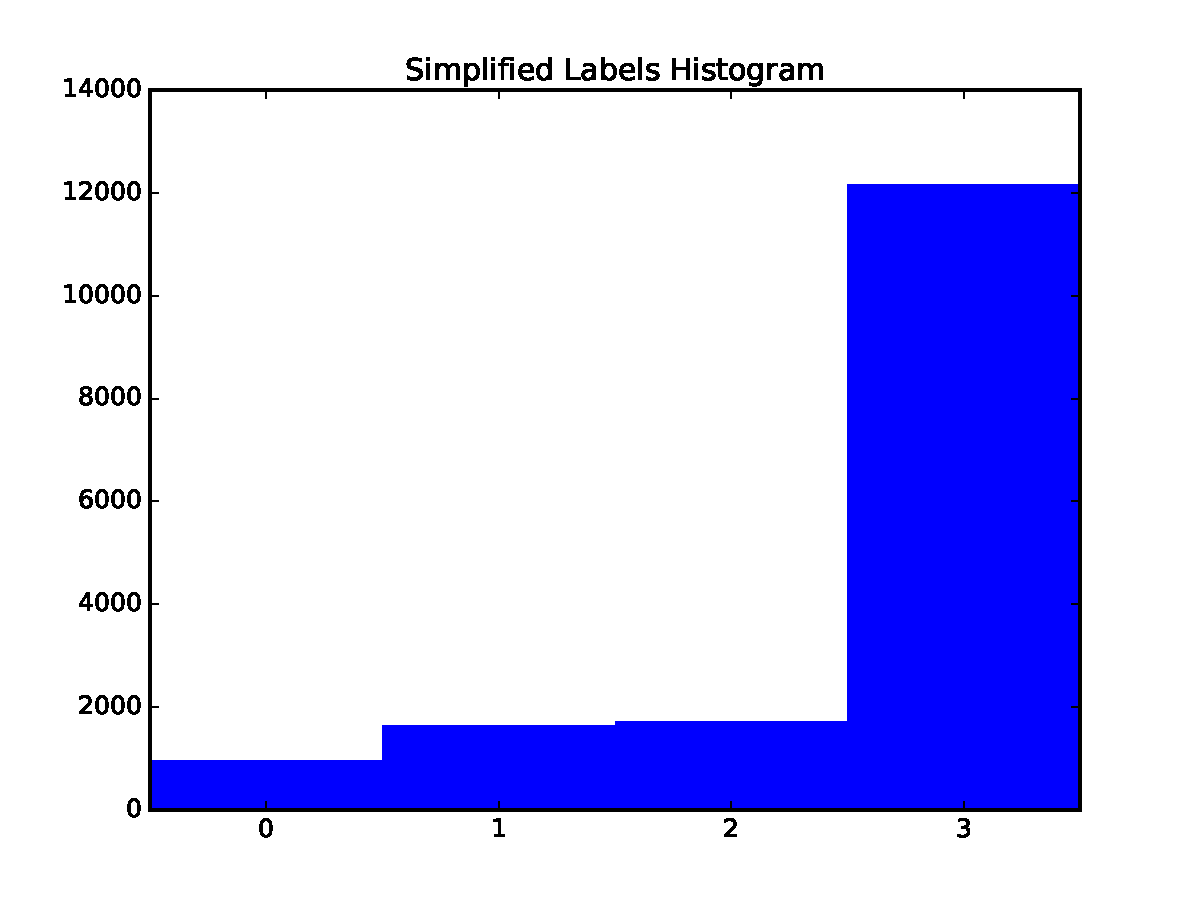
\includegraphics[width=\linewidth]{hist_simple_labels.pdf}
        \caption{Distribution of simplified labels in original dataset}
        \label{fig:singlelabeldistr}
    \end{minipage}
    \hfill
    \begin{minipage}{.49\linewidth}
        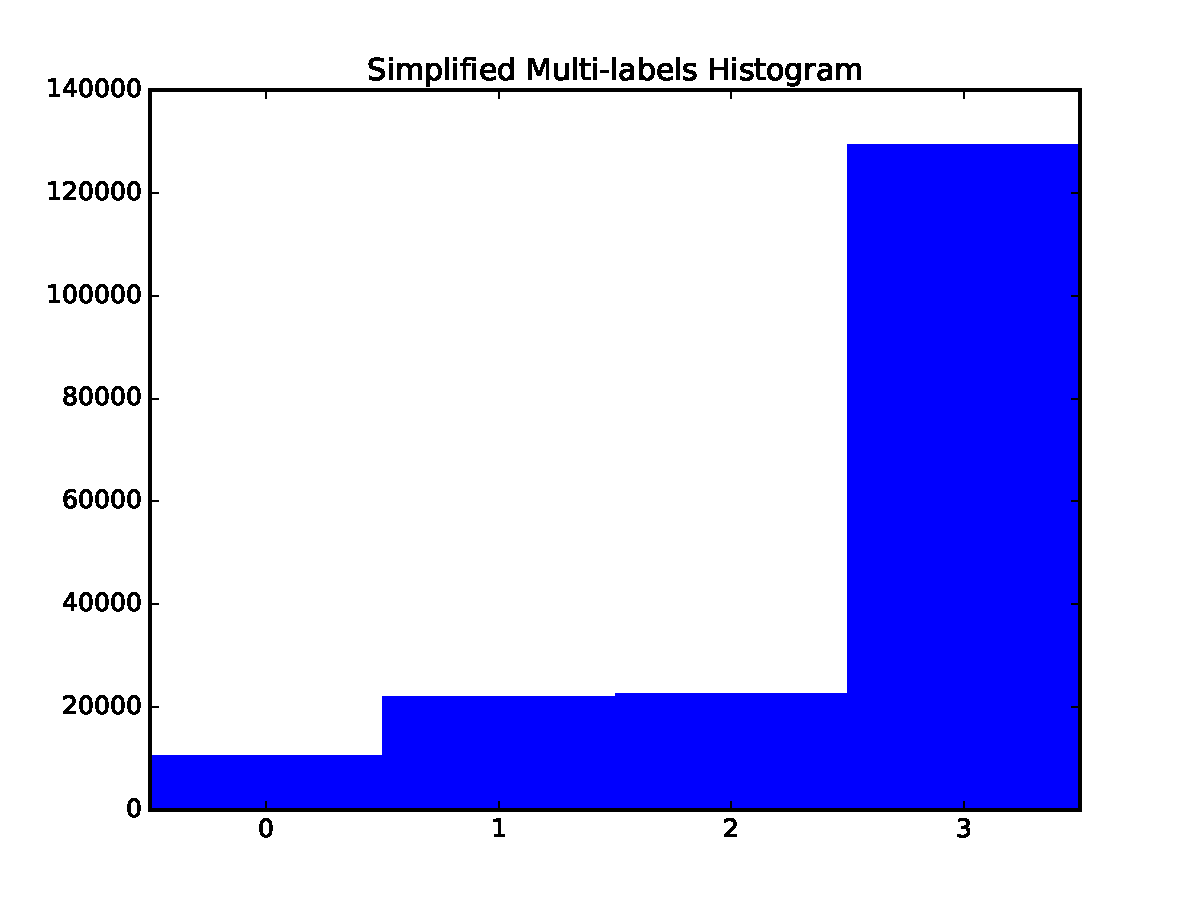
\includegraphics[width=\linewidth]{hist_simple_multi_labels.pdf}
        \caption{Distribution of simplified labels in multi-label outputs}
        \label{fig:multilabeldistr}
    \end{minipage}
\end{figure}

\subsection{Coordinates as features}
Due to the abundant bathymetry data that was available in the form of depth, rugosity and aspect at each available data point, there was reason not to include the coordinates themselves in the feature space. Whilst it does make sense that in a natural environment, areas that were spatially near to one another would also have similar properties, this should not be relied upon, and other intrinsic properties should be the basis upon which predictions are made. Forming predictions on the full query dataset using a random forest supports this notion quite strongly - whilst 10-fold cross validation using the coordinates as features had a notably higher F-score of 0.61 compared to 0.40 without, the unnaturally straight split between the left and right segments over a 12km region suggests that the predictive map is flawed. \todo{(argument here alone is weak. for simplified labels using coords is still much better by a similar margin, do some reading to back this up properly)}

\begin{figure}[H]
    \begin{minipage}{.49\linewidth}
        \includegraphics[width=\linewidth]{full_predictions_randomforest.pdf}
        \caption{Full predictive map using Random Forests including coordinates as features}
        \label{fig:rf_w_coords_preds}
    \end{minipage}
    \hfill
    \begin{minipage}{.49\linewidth}
        \includegraphics[width=\linewidth]{full_predictions_randomforest_nocoords.pdf}
        \caption{Full predictive map using Random Forests excluding coordinates as features}
        \label{fig:rf_wo_coords_preds}
    \end{minipage}
\end{figure}


\subsection{Subsampling for Gaussian Process experiments}

Due to the $O(n^3)$ complexity of training a Gaussian Process Classifier, using all $16502$ points was infeasible, so it was necessary to use only a subsample of the training data. As can be seen in the above histograms \todo{(reference the figure instead. may need to combine them into one)}, the distribution of classes in both the simplified and non-simplified versions was very uneven. As a result of this skew, randomly sampling the the training data to fit our GP classifier against resulted in worse results than samplying an equal \textit{number} of points for each class. To obtain a reasonably well-performing set of 1000 points (the number chosen to obtain a balance between performance and time required), 10-fold cross validation was performed on random sets of 1000 with each class sampled equally, and the best set chosen after 200 runs of random subsampling.

\section{Illustrative Example}

The differences between a Gaussian Process that provides the probability distribution of possible labels compared to the Dirichlet Multinomial Regressor that provides the distribution of actual labels at a point, are highlighted in the illustrative example below. Note that three clusters were synthesised, with clusters A, B containing $0.7:0.3$ and $0.3:0.7$ average ratios in label mix per point respectively, while cluster C contained an even $0.5:0.5$ average split, where cluster had $100$ points. The colours on the overall plot are only representative of the \textbf{most} common label at each point - the actual distributions at each point are shown in the graphs following it.

% \todo{generate toy example with a mixed label A,B region and separate regions of mostly A, mostly B respectively}

\begin{figure}[H]
    \includegraphics[scale=0.7]{toydataplot.pdf}
    \caption{Plots of the three clusters, with labels taking on the argmax of each point}
    \label{fig:toyplot}
\end{figure}

\begin{figure}[H]
    \includegraphics[trim={0 2cm 0 2cm}]{toyplot_hist_distr_legend.pdf}
    \caption{Legend/axes for the following histogram plots showing distribution of labels at each point}
    \label{fig:toyplothist_legend}
\end{figure}

\begin{figure}[H]
    \begin{minipage}{.49\linewidth}
        \includegraphics[width=\linewidth]{toy_clusterA_distr.pdf}
        \caption{Label distribution of cluster A}
        \label{fig:toyclusterA}
    \end{minipage}
    \hfill
    \begin{minipage}{.49\linewidth}
        \includegraphics[width=\linewidth]{toy_clusterB_distr.pdf}
        \caption{Label distribution of cluster B}
        \label{fig:toyclusterB}
    \end{minipage}
    \begin{minipage}{.49\linewidth}
        \includegraphics[width=\linewidth]{toy_clusterC_distr.pdf}
        \caption{Label distribution of cluster C}
        \label{fig:toyclusterC}
    \end{minipage}
\end{figure}

In this example, the GP and DM models were each trained on half of each cluster, and made to predict the other half. However, as a standard GPC can only have single label inputs and outputs, a approximation/simplification was made for the purpose of calculating average error, whereby the label was simply taken to be the most frequently occurring label at any given point. While this is a reasonable simplification for clusters A, B as the dominant label has majority share, this is not the case for C, as the split between the two labels per point in the cluster is exactly even. In an initial attempt to counter this, multi-task GPs were considered as a means of making a \textit{fairer} comparison between a GP and DM, but the idea was ultimately discarded as it was not fit for purpose, one of the primary issues being that the model does not inherently restrict the outputs of a given datapoint to sum to $1$, instead being at the mercy of the parameters of the GP. The results and plots for this example are below, and figures displayed were taken from an average of $20$ runs.

\begin{tabular}{|C{4cm}|C{4cm}|c|}
    \hline
    & Dirichlet Multinomial Regression RMSE* & Gaussian Process Classifier (argmax) RMSE \\\hline
    Original data & 0.070179271314358999 & 0.26833333333333337 \\\hline
    Quadratic-space projection & 0.065630111843395234 & 0.43433333333333335 \\\hline
    Cubic-space projection & 0.29019235800882354 & 0.43725490196076466 \\\hline
\end{tabular}
\begingroup
\tiny{RMSE - root mean squared error}
\endgroup

As can be seen from the above overvise, the DM performed best when projecting the data to quadratic space, while the GPC didbest on the original data as-is. This was taken into account for the plots below for the DM and GP respectively, which used an instance of the more favourably performing processed data. Note that the exact probabilities provided by the GP are hown in the following plots, in contrast to the argmax taken for error-calculation purposes.

\begin{figure}[H]
    \includegraphics[scale=0.6]{toy_dm_pred_plot0.pdf}
    \caption{DM Label distribution of label 0}
    \label{fig:toylabel0}
\end{figure}
\begin{figure}[H]
    \includegraphics[scale=0.6]{toy_dm_pred_plot1.pdf}
    \caption{DM Label distribution of label 1}
    \label{fig:toylabel1}
\end{figure} 
%\todo{dm - sitting on averages in each cluster. cause for concern?}

\begin{figure}[H]
    \includegraphics[scale=0.6]{gp_with_vars0.pdf}
    \caption{OvR GP performance with variance for label 0}
    \label{fig:toylabel0}
\end{figure}
\begin{figure}[H]
    \includegraphics[scale=0.6]{gp_with_vars1.pdf}
    \caption{OvR GP performance with variance for label 1}
    \label{fig:toylabel1}
\end{figure} 

As we can see, the DM performed notably better than the GP, though this is admittedly a rather simple example that assumes we have a sufficient amount of data from the \textit{three} possible habitat clusters - A by itself, B by itself, and a homogeneous mix of A and B.

From this basic example, it is apparent that in the area where there is an even mix of labels A, B, the Gaussian Process' predictions are both noisy and very uncertain about their predictions, where human intervention would be required to observe the fact that it is in fact a consistent mix of both. In contrast, the dirichlet multinomial regressor is more confident in the fact that that area does in fact have a mix of labels.
